There are various different metrics that can be used for evaluating the output
of a classifier or segmentation algorithm, many of which we have seen in previous
sections. I was analyse a few of these evaluations of results so that I can use
them as a reference to apply to my own experiments. I will also look into some
problems associated with evaluating models.

\subsection{Research into Diagnosing Errors in Object Detectors}
There has been some research into the question of how to evaluate object
detectors, one of which I will discuss in detail \textcite{diagnosingErrors}.
This paper in question "analyzes the influences of object characteristics on
detection performance and the frequency and impact of different types of false
positives" \textcite{diagnosingErrors}. They found that there were many effects
that had influence on detectors as follows:
\begin{itemize}
    \item{occlusion}
    \item{size}
    \item{aspect ratio}
    \item{visibility of parts}
    \item{viewpoint}
    \item{localization error}
    \item{confusion with semantically similar objects}
    \item{confusion with other labeled objects}
    \item{confusion with background}
\end{itemize}

The research team goes on to analyse false positives in object detectors.
Localization errors were a large factor. This is were bounding boxes overlap to
other objects in the image. Confusion with similar objects had a large influence
on false positives also by which, for example, a dog detector had a high score
for a cat \textcite{diagnosingErrors}. Confusion with dissimilar objects and
confusion with background are the categories of the rest of the false positives
they measured.

In conclusion the team would that "Most false positives are due to misaligned
detection windows or confusion with similar objects"
\textcite{diagnosingErrors}. They had some recommendations towards improves
detectors as follows:
\begin{itemize}
	\item{Smaller objects are less likely to be detected}
	\item{Localization could be improved}
	\item{Reduce confusion with similar categories}
	\item{Robustness to object variation}
	\item{More detailed analysis}
\subsection{Detection Average Precision}
See \ref{fig:dap}.
\begin{figure}
	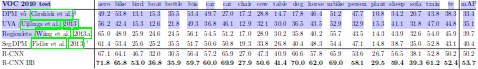
\includegraphics[width=150mm,scale=0.5]{DAP}
	\caption{Detection Average Precision \textcite{donahue}}
    \label{fig:dap}
\end{figure}

\subsection{Mean Average Precision}
See \ref{fig:MAP}.
		\begin{figure}
			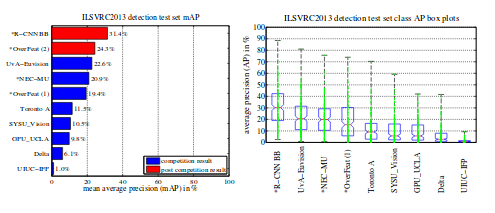
\includegraphics[width=150mm,scale=0.5]{MAP}
			\caption{Mean Average Precision \textcite{donahue}}
			\label{fig:MAP}
		\end{figure}
		
\subsection{Distribution of top-ranked false positives}
See \ref{fig:DFP}.
		\begin{figure}
			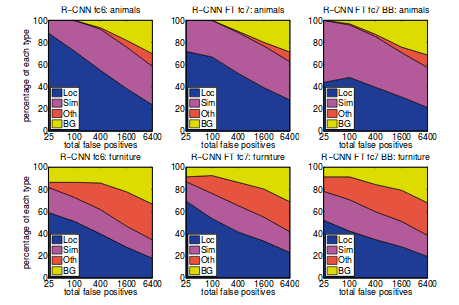
\includegraphics[width=150mm,scale=0.5]{DFP}
			\caption{Distribution of top-ranked false positives \textcite{donahue}}
			\label{fig:DFP}
		\end{figure}
		

\subsection{Segmentation Mean Accuracy}
See \ref{fig:SMP}.
		\begin{figure}
			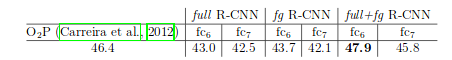
\includegraphics[width=150mm,scale=0.5]{SMP}
			\caption{Segmentation Mean Accuracy \textcite{donahue}}
			\label{fig:SMP}
		\end{figure}
		

\subsection{Per-category segmentation accuracy}
See \ref{fig:PCATSA}.
		\begin{figure}
			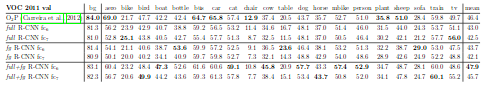
\includegraphics[width=150mm,scale=0.5]{PCATSA}
			\caption{Per-category segmentation accuracy \textcite{donahue}}
			\label{fig:PCATSA}
		\end{figure}
		

\subsection{Per-class segmentation accuracy}
\See \ref{fig:PCLASSA}.
		\begin{figure}
			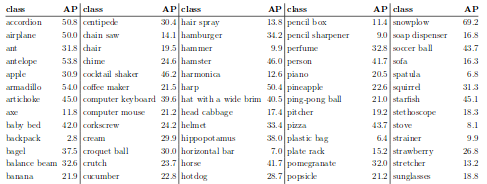
\includegraphics[width=150mm,scale=0.5]{PCLASSSA}
			\caption{Per-class segmentation accuracy \textcite{donahue}}
			\label{fig:PCLASSA}
		\end{figure}
		

